\section{Przemysław Rutyna} 
\label{sec:prutyna}
Przykładowy wielomian : 
\[ ax^3 + bx^2 + cx + d\]
Zdjęcie : 
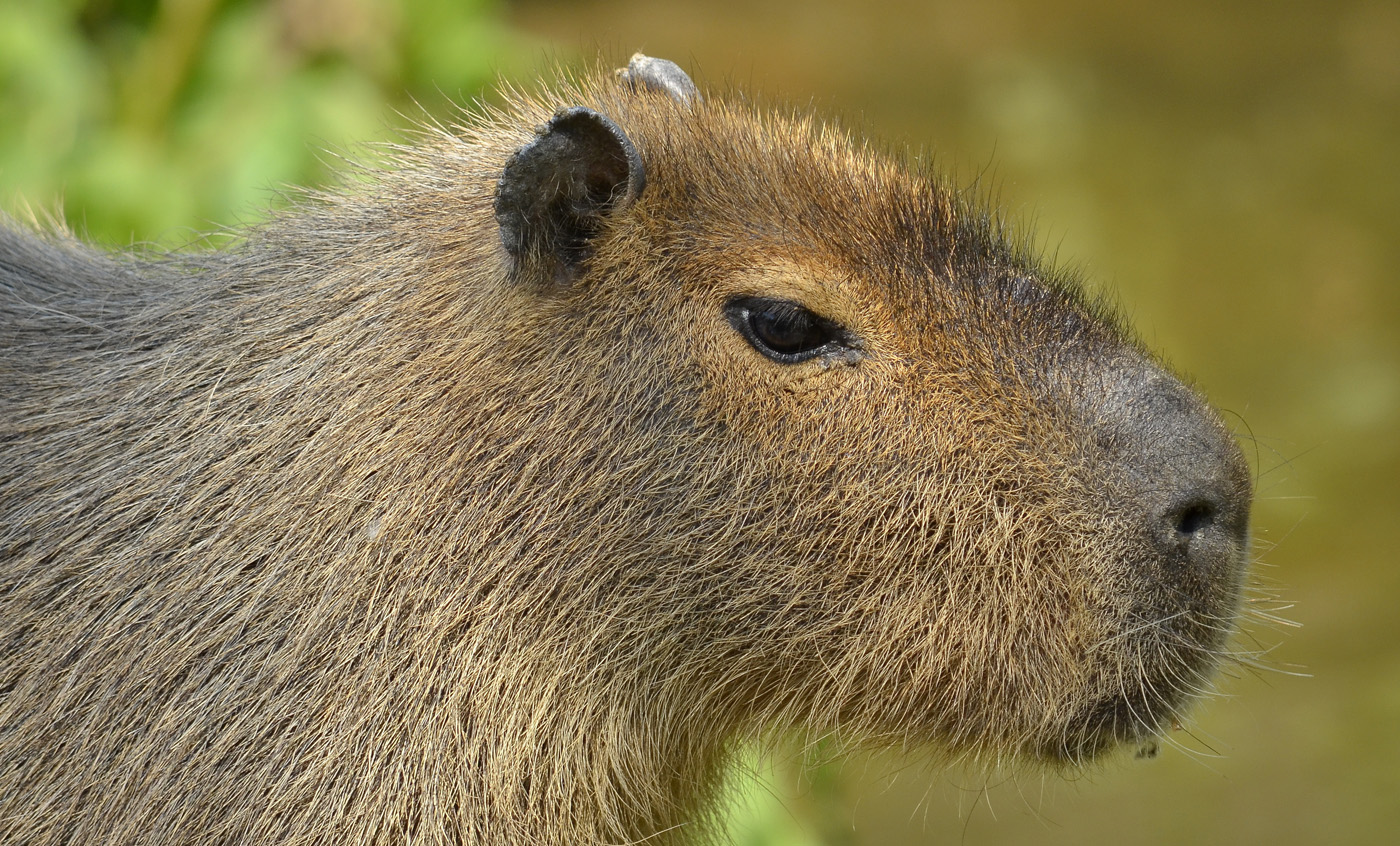
\includegraphics{pictures/Pszym/cap.jpg}
\begin{table}
\begin{tabular}{lllll}
a1 & b1 & c1 & d1 & e1 \\
a2 & b2 & c2 & d2 & e2 \\
a3 & b3 & c3 & d3 & e3 \\
a4 & b4 & c4 & d4 & e4
\end{tabular}
\end{table}
\begin{itemize}
  \item Pierwszy element listy.
  \item Drugi element listy.
  \item Trzeci element listy.
\end{itemize}
\begin{enumerate}
  \item Pierwszy element listy tym razem numerowanej.
  \item Czwarty element listy tym razem numerowanej.
  \item Trzeci element listy tym razem numerowanej.
\end{enumerate}
\begin{center}
\textbf{Nunc nibh lorem, feugiat sed convallis ut, accumsan eu ligula. In consectetur efficitur facilisis.} Praesent bibendum lacinia quam, vitae lacinia nisi molestie sed. Donec vel risus eu odio semper pretium. Pellentesque posuere turpis vitae fermentum placerat. Duis vitae neque id ante interdum hendrerit. Fusce vulputate erat nec dui pulvinar, sodales fermentum nisl accumsan. Integer sed neque nulla. Cras vitae volutpat nunc, ut tempor libero. Proin id pharetra quam. Nunc vitae massa ex.

\textit{In auctor sollicitudin imperdiet. Aenean eget leo ut erat sollicitudin dictum a vitae massa.} Fusce purus neque, laoreet eu libero vel, aliquet pharetra dui. Etiam sed lacus ac ipsum venenatis bibendum et lacinia nibh. Vestibulum a mollis est, et luctus arcu. Cras a porta purus. Sed sed purus odio. Maecenas et turpis et nibh suscipit sollicitudin eget feugiat neque. Vivamus non pulvinar velit. Curabitur fringilla nunc felis, non venenatis ligula semper ut. Nulla mattis, tellus eget rutrum scelerisque, nunc lorem pellentesque sem, ullamcorper pretium lorem erat et velit. Phasellus vehicula dapibus rutrum. Proin sit amet lorem vitae nunc finibus placerat nec porttitor orci. Nulla lacus nibh, condimentum vel elit et, egestas accumsan ante. Praesent in lorem varius, porta tellus eget, bibendum augue. Donec ex purus, tincidunt et dignissim a, pellentesque mollis urna.
\end{center}
\begin{figure}[h!]
  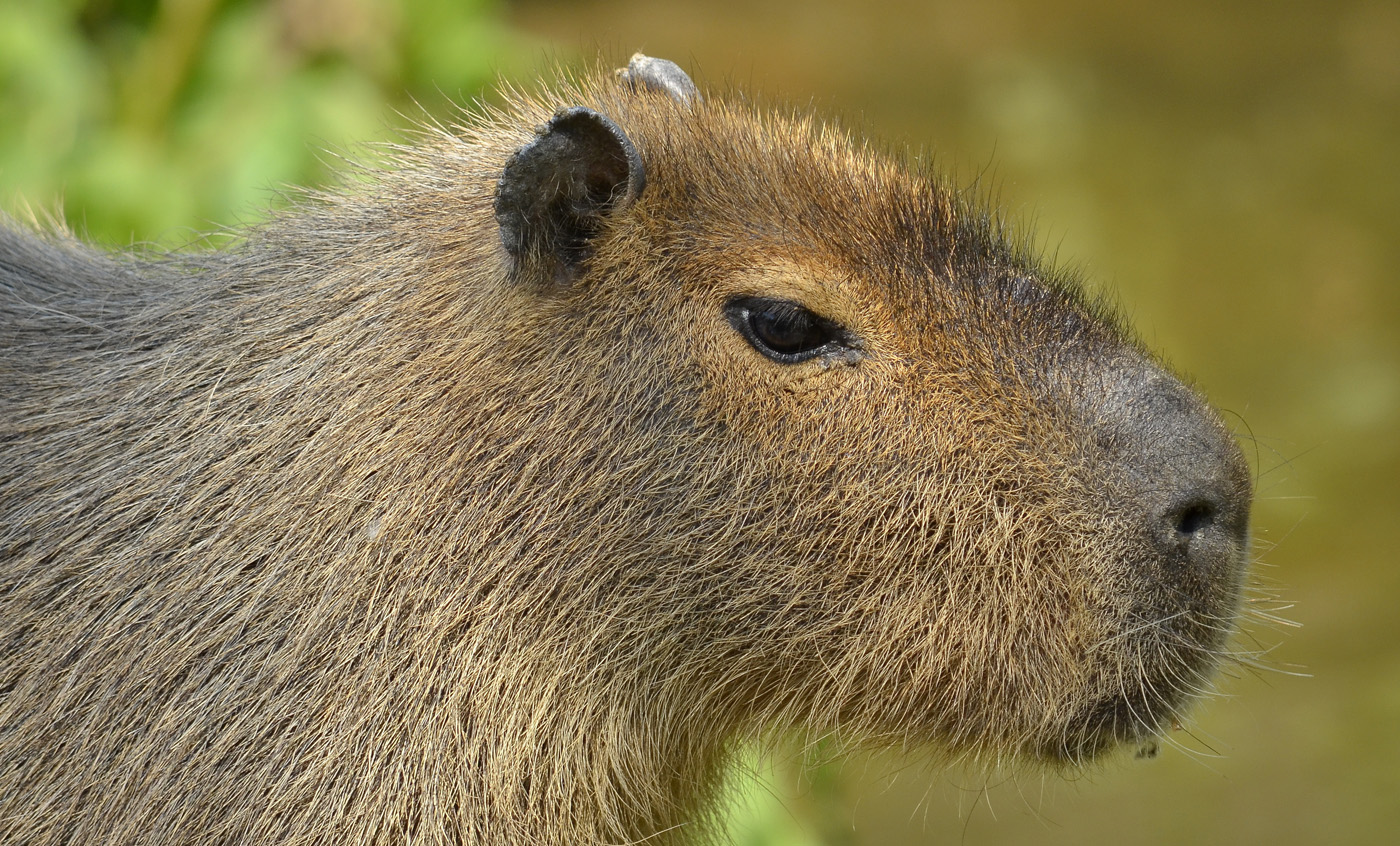
\includegraphics[scale=1.3]{pictures/Pszym/cap.jpg}
  \caption{Capibara}
  \label{fig:capibara}
\end{figure}